\documentclass[11pt]{article}
\usepackage{geometry}                % See geometry.pdf to learn the layout options. There are lots.
\geometry{letterpaper}                   % ... or a4paper or a5paper or ... 
%\geometry{landscape}                % Activate for for rotated page geometry
%\usepackage[parfill]{parskip}    % Activate to begin paragraphs with an empty line rather than an indent
\usepackage{graphicx}
\usepackage{amssymb,amsmath}
\usepackage{epstopdf}
\usepackage{pgf}
\usepackage{pgfpages}
\usepackage{tikz}
\usetikzlibrary{arrows,backgrounds}
\usepgflibrary{shapes}
\DeclareGraphicsRule{.tif}{png}{.png}{`convert #1 `dirname #1`/`basename #1 .tif`.png}
\pagestyle{empty}


\begin{document}

 % Hexahedron node numbering
  \begin{center}
    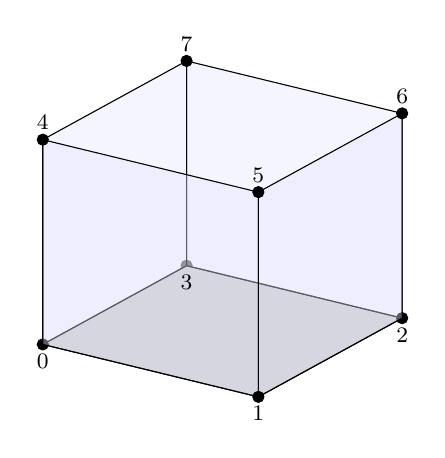
\begin{tikzpicture}[join=round] % Hex with 8 nodes
        \filldraw(-.456,.833) circle (2pt);
        \filldraw[fill=black!20](2.282,.167)--(-.456,.833)--(-2.282,-.167)--(.456,-.833)--cycle;
        \filldraw[fill=blue!10,fill opacity=0.4](-2.282,2.433)--(-2.282,-.167)--(-.456,.833)--(-.456,3.433)--cycle;
        \filldraw[fill=blue!10,fill opacity=0.4](-.456,3.433)--(-.456,.833)--(2.282,.167)--(2.282,2.767)--cycle;
        \filldraw(-.456,3.433) circle (2pt);
        \filldraw(2.282,.167) circle (2pt);
        \filldraw[fill=blue!10,fill opacity=0.4](2.282,2.767)--(2.282,.167)--(.456,-.833)--(.456,1.767)--cycle;
        \filldraw(-2.282,-.167) circle (2pt);
        \filldraw[fill=blue!10,fill opacity=0.4](.456,1.767)--(.456,-.833)--(-2.282,-.167)--(-2.282,2.433)--cycle;
        \filldraw(2.282,2.767) circle (2pt);
        \filldraw(-2.282,2.433) circle (2pt);
        \filldraw(.456,-.833) circle (2pt);
        \filldraw(.456,1.767) circle (2pt);
        \fill[black,font=\footnotesize]
                (-2.282,-.167) node [below] {0}
                (.456,-.833) node [below] {1}
                (2.282,.167) node [below] {2}
                (-.456,.833) node [below] {3}
                (-2.282,2.433) node [above] {4}
                (.456,1.767) node [above] {5}
                (2.282,2.767) node [above] {6}
                (-.456,3.433) node [above] {7};
     \end{tikzpicture}
     \hspace{1cm}
    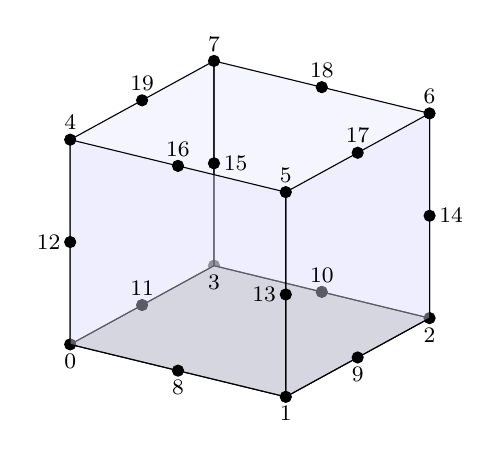
\begin{tikzpicture}[join=round] % Hex with 20 nodes
        \filldraw(-.456,.833) circle (2pt);
        \filldraw[fill=black!20](2.282,.167)--(-.456,.833)--(-2.282,-.167)--(.456,-.833)--cycle;
        \filldraw[fill=blue!10,fill opacity=0.4](-2.282,2.433)--(-2.282,-.167)--(-.456,.833)--(-.456,3.433)--cycle;
        \filldraw[fill=blue!10,fill opacity=0.4](-.456,3.433)--(-.456,.833)--(2.282,.167)--(2.282,2.767)--cycle;
        \filldraw(-.456,2.133) circle (2pt);
        \filldraw(.913,.5) circle (2pt);
        \filldraw(-.456,3.433) circle (2pt);
        \filldraw(-1.369,.333) circle (2pt);
        \filldraw(2.282,.167) circle (2pt);
        \filldraw[fill=blue!10,fill opacity=0.4](2.282,2.767)--(2.282,.167)--(.456,-.833)--(.456,1.767)--cycle;
        \filldraw(.913,3.1) circle (2pt);
        \filldraw(2.282,1.467) circle (2pt);
        \filldraw(-1.369,2.933) circle (2pt);
        \filldraw(-2.282,-.167) circle (2pt);
        \filldraw[fill=blue!10,fill opacity=0.4](.456,1.767)--(.456,-.833)--(-2.282,-.167)--(-2.282,2.433)--cycle;
        \filldraw(2.282,2.767) circle (2pt);
        \filldraw(1.369,-.333) circle (2pt);
        \filldraw(-2.282,1.133) circle (2pt);
        \filldraw(-.913,-.5) circle (2pt);
        \filldraw(-2.282,2.433) circle (2pt);
        \filldraw(1.369,2.267) circle (2pt);
        \filldraw(.456,-.833) circle (2pt);
        \filldraw(-.913,2.1) circle (2pt);
        \filldraw(.456,.467) circle (2pt);
        \filldraw(.456,1.767) circle (2pt);
        \fill[black,font=\footnotesize]
                (-2.282,-.167) node [below] {0}
                (.456,-.833) node [below] {1}
                (2.282,.167) node [below] {2}
                (-.456,.833) node [below] {3}
                (-2.282,2.433) node [above] {4}
                (.456,1.767) node [above] {5}
                (2.282,2.767) node [above] {6}
                (-.456,3.433) node [above] {7}
                (-.913,-.5) node [below] {8}
                (1.369,-.333) node [below] {9}
                (.913,.5) node [above] {10}
                (-1.369,.333) node [above] {11}
                (-2.282,1.133) node [left] {12}
                (.456,.467) node [left] {13}
                (2.282,1.467) node [right] {14}
                (-.456,2.133) node [right] {15}
                (-.913,2.1) node [above] {16}
                (1.369,2.267) node [above] {17}
                (.913,3.1) node [above] {18}
                (-1.369,2.933) node [above] {19};
    \end{tikzpicture}
  \end{center}
  \begin{center} {(a) \hspace{5cm} (b)} \end{center}
   \begin{center}
      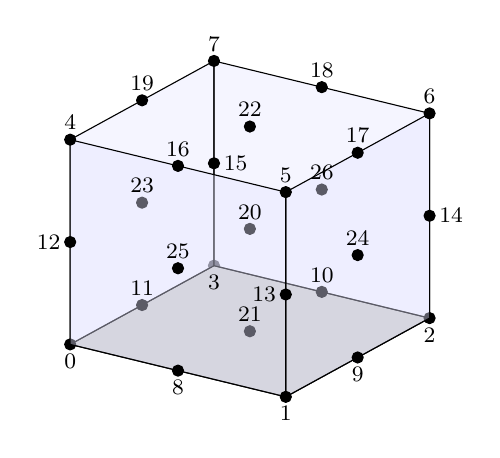
\begin{tikzpicture}[join=round]
          \filldraw(-.456,.833) circle (2pt);
          \filldraw[fill=black!20](2.282,.167)--(-.456,.833)--(-2.282,-.167)--(.456,-.833)--cycle;
          \filldraw[fill=blue!10,fill opacity=0.4](-2.282,2.433)--(-2.282,-.167)--(-.456,.833)--(-.456,3.433)--cycle;
          \filldraw[fill=blue!10,fill opacity=0.4](-.456,3.433)--(-.456,.833)--(2.282,.167)--(2.282,2.767)--cycle;
          \filldraw(-.456,2.133) circle (2pt);
          \filldraw(.913,.5) circle (2pt);
          \filldraw(-.456,3.433) circle (2pt);
          \filldraw(-1.369,.333) circle (2pt);
          \filldraw(.913,1.8) circle (2pt);
          \filldraw(2.282,.167) circle (2pt);
          \filldraw[fill=blue!10,fill opacity=0.4](2.282,2.767)--(2.282,.167)--(.456,-.833)--(.456,1.767)--cycle;
          \filldraw(-1.369,1.633) circle (2pt);
          \filldraw(.913,3.1) circle (2pt);
          \filldraw(0,0) circle (2pt);
          \filldraw(2.282,1.467) circle (2pt);
          \filldraw(-1.369,2.933) circle (2pt);
          \filldraw(-2.282,-.167) circle (2pt);
          \filldraw(0,1.3) circle (2pt);
          \filldraw[fill=blue!10,fill opacity=0.4](.456,1.767)--(.456,-.833)--(-2.282,-.167)--(-2.282,2.433)--cycle;
          \filldraw(2.282,2.767) circle (2pt);
          \filldraw(1.369,-.333) circle (2pt);
          \filldraw(-2.282,1.133) circle (2pt);
          \filldraw(0,2.6) circle (2pt);
          \filldraw(-.913,-.5) circle (2pt);
          \filldraw(1.369,.967) circle (2pt);
          \filldraw(-2.282,2.433) circle (2pt);
          \filldraw(-.913,.8) circle (2pt);
          \filldraw(1.369,2.267) circle (2pt);
          \filldraw(.456,-.833) circle (2pt);
          \filldraw(-.913,2.1) circle (2pt);
          \filldraw(.456,.467) circle (2pt);
          \filldraw(.456,1.767) circle (2pt);
          \fill[black,font=\footnotesize]
                (-2.282,-.167) node [below] {0}
                (.456,-.833) node [below] {1}
                (2.282,.167) node [below] {2}
                (-.456,.833) node [below] {3}
                (-2.282,2.433) node [above] {4}
                (.456,1.767) node [above] {5}
                (2.282,2.767) node [above] {6}
                (-.456,3.433) node [above] {7}
                (-.913,-.5) node [below] {8}
                (1.369,-.333) node [below] {9}
                (.913,.5) node [above] {10}
                (-1.369,.333) node [above] {11}
                (-2.282,1.133) node [left] {12}
                (.456,.467) node [left] {13}
                (2.282,1.467) node [right] {14}
                (-.456,2.133) node [right] {15}
                (-.913,2.1) node [above] {16}
                (1.369,2.267) node [above] {17}
                (.913,3.1) node [above] {18}
                (-1.369,2.933) node [above] {19}
                (0,1.3) node [above] {20}
                (0,0) node [above] {21}
                (0,2.6) node [above] {22}
                (-1.369,1.633) node [above] {23}
                (1.369,.967) node [above] {24}
                (-.913,.8) node [above] {25}
                (.913,1.8) node [above] {26};
    \end{tikzpicture}
  \end{center}
  \begin{center} 
   (c)  
   \end{center}

\end{document}  
